\documentclass[11pt, fleqn]{article}

\usepackage[usenames,dvipsnames,svgnames,table]{xcolor}
\usepackage{amsmath}
\usepackage{amsfonts}
\usepackage[margin=1in]{geometry} % To set the margin widths
\usepackage{graphicx}
\usepackage{listings}
\usepackage{multirow}
\usepackage{tabularx}
\usepackage{varioref}
\usepackage[noabbrev,capitalize]{cleveref}
\usepackage[group-separator={,}]{siunitx}
\usepackage{subcaption}
\usepackage{titlesec}
\usepackage{lscape}
\usepackage{bm}
\usepackage{chngpage}
\usepackage[titletoc,toc,title]{appendix}

\renewcommand\thesection{\arabic{section}}
\renewcommand\thesubsection{\thesection\alph{subsection}}

\lstset{
  frame=single,
  basicstyle=\ttfamily,% print whole listing small
  language=R,
  aboveskip=3mm,
  belowskip=3mm,
  showstringspaces=false,
  columns=flexible,
  numbers=none,
  commentstyle=\color{ForestGreen},
  stringstyle=\color{Maroon},
  breaklines=true,
  breakatwhitespace=true,
  tabsize=2,
  literate={<-}{{$\gets$}}1 {~}{{$\sim$}}1
}

\sisetup{output-exponent-marker=\textsc{e}}

\setlength{\parskip}{12pt} % Sets a blank line in between paragraphs
\setlength\parindent{0pt} % Sets the indent for each paragraph to zero

\begin{document}

\title{Homework \#1\\
Digital and Algorithmic Marketing (37304-01)}
\author{
Brian Chingono, Will Clark, Matthew DeLio, Yoni Sarason, Jonathan Stevens \and (\textbf{Group \#8})\\
University of Chicago Booth School of Business}

\maketitle

\section{Data Exploration}

Prior to approaching the decisions of whether we should go with the new DMP, and whether we should go after the entire target file audience, we first conducted some data exploration:  
\begin{itemize}

\item For all customers in our existing customer data set, median spending is 0 dollars and mean spending is 2.902 dollars. There are 5,000 customer observations in this data set.

\item We determined that it would be more useful to look at the subset of customers in the existing dataset who actually had spending greater than 0 dollars.  Among those with positive spending, the median and mean spending was 29.94 dollars and 97.37 dollars, respectively.  \vref{fig:cust_spend_cdf} shows a Cumulative Distribution Function of spending for the subset of customers with spending greater than zero. \vref{fig:cust_spend_hist} shows a histogram of spending by customers with spending greater than zero.  

\item The target dataset contains 19,686 observations and also has median and mean spending customer spending near zero for all observations.  However, among only the potential customers in the target data set that have nonzero spending, the median and mean levels of spending are 35.78 dollars and 59.82 dollars, respectively. 

\item Given the cost of 3.25 dollars per match from the target data set, the expected profit from blanketing the entire target dataset is -3,263.17 dollars.  Thus it appears that applying a matching algorithm may be a useful tool in segmenting the market and achieving positive profits.  

\end{itemize}

% Note this CDF plot is for customers that did spend at least something
\begin{figure}[!htb]
  \centering
  \caption{CDF of Customer Spending}
  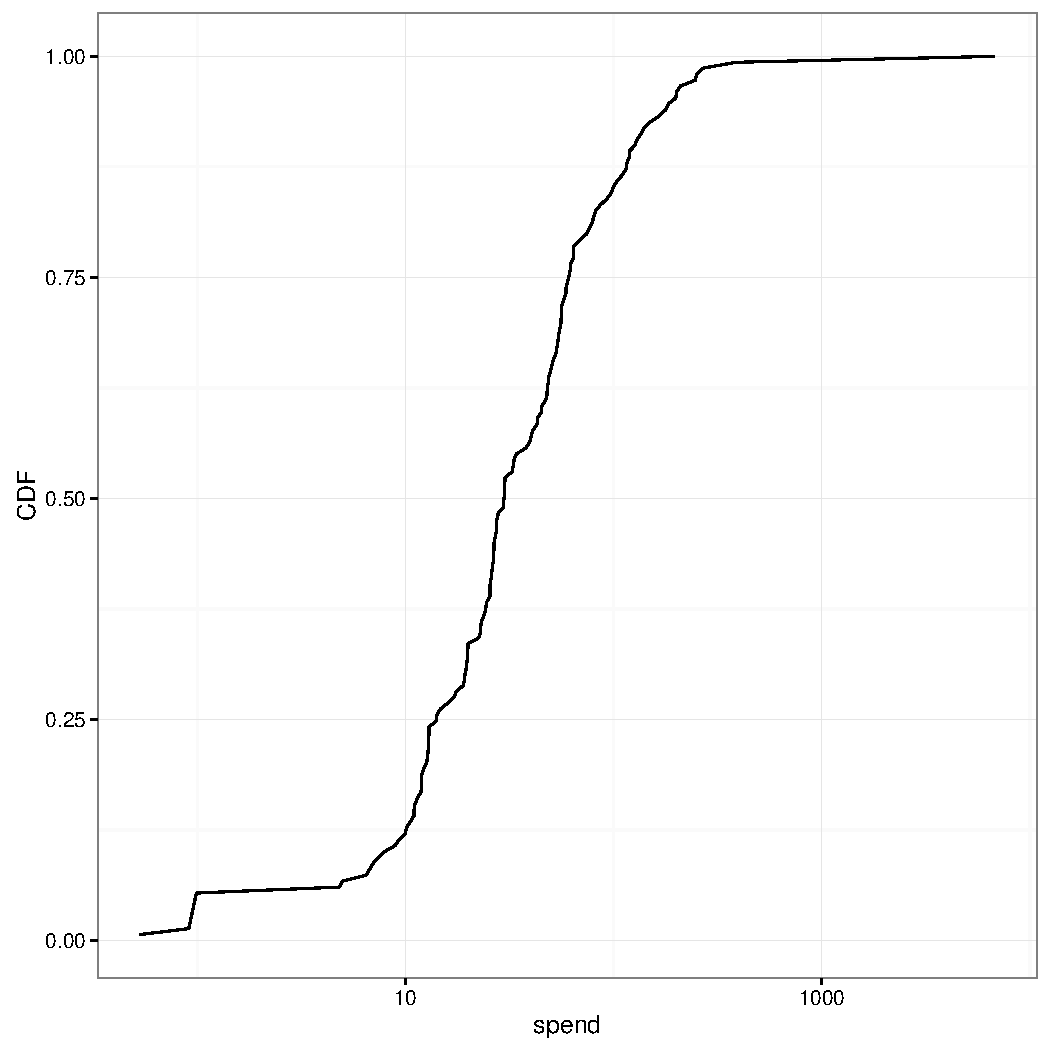
\includegraphics[scale=.5]{cust_spend_cdf.pdf}
  \label{fig:cust_spend_cdf}
\end{figure}

% Again, this is for actual customers that spent something.
% we might want to only include the histogram or cdf.
\begin{figure}[!htb]
  \centering
  \caption{Histogram of Customer Spending}
  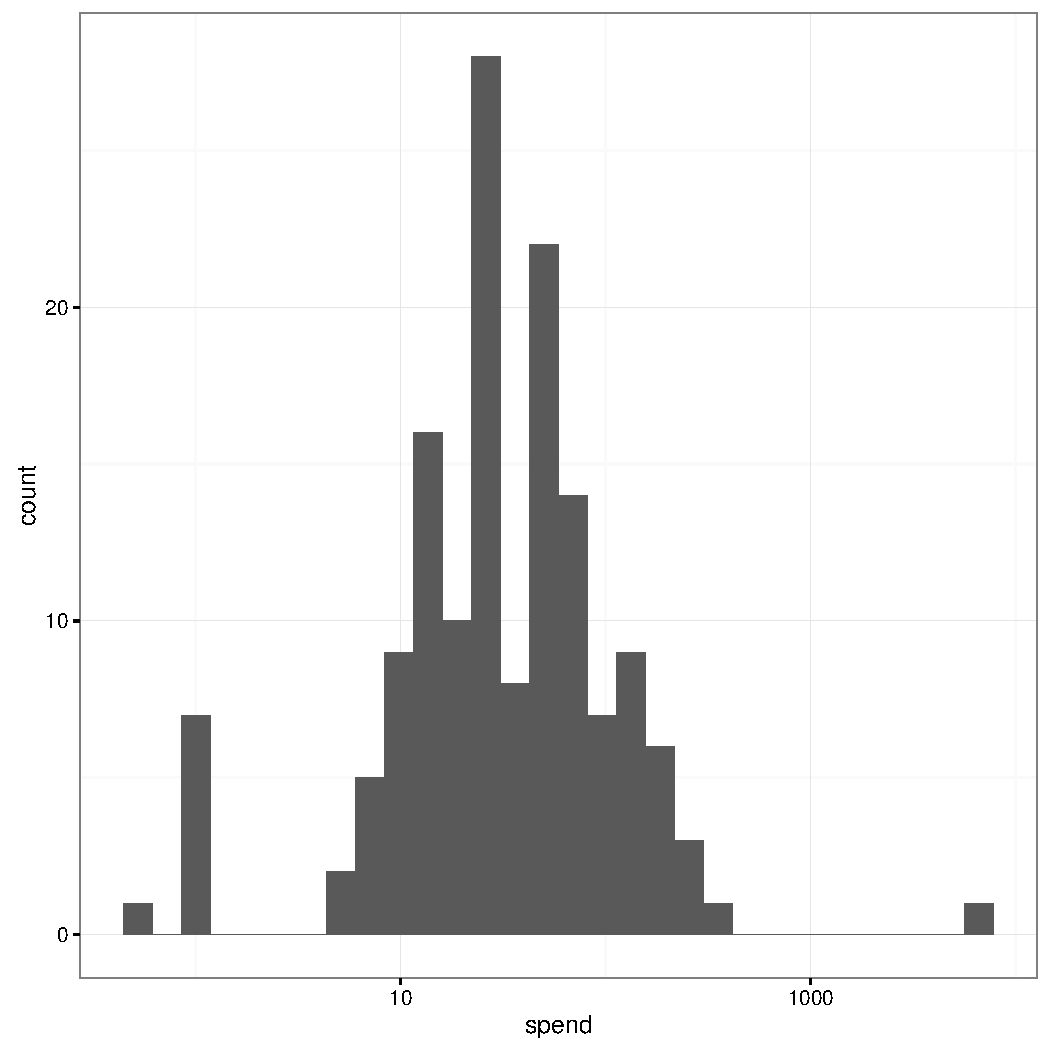
\includegraphics[scale=.5]{cust_spend_hist.pdf}
  \label{fig:cust_spend_hist}
\end{figure}


\section{K-Means Matching}

We first built a matching algorithm using k-means clustering. We used the following algorithm:
\begin{itemize}
\item Find every fifth quantile of non-zero customer spending (see \cref{tab:cutoffs} in the Appendix). We will define a valuable customer as one who spends at or above the quantile level. For each quantile:
\begin{itemize}
\item Use a k-means algorithm to break the customers into $k$ clusters, where we search over a range of $k$ from 1 to 20. For each $k$ number of clusters:
\begin{itemize}
\item Define the "matching" group in the target set as the nearest $j$ clusters, where we vary $j$ from 1 to $k$. For example, suppose that we use $k=10$ clusters. Then we would define the "match" data set as the nearest cluster, then the nearest two clusters, then the nearest three clusters, etc.
\end{itemize}
\end{itemize}
\item For each combination of the quantile cutoff, $k$ clusters, and $j$ matches, calculate the profitability of targeting the resulting match data set. The optimal set of parameters is that which maximizes profitability.
\end{itemize}
We use this algorithm to find the most profitable targeting strategy in the original data set and the data set that includes the ecom\_index. We show the results in \cref{fig:kmeans_profit1} and \cref{fig:kmeans_profit2}, respectively.

In the first case, the optimal cutoff for defining a valuable customer is one who spends more than \$127.15, which is the 90th percentile of non-zero spending. If we break the target data into 20 clusters and match on only the nearest cluster, we can make a profit of only \$283.

In the second case, the optimal cutoff for customer value is the 95th percentile, or \$192.63. In this case, we use $k=18$ clusters and again match on only the nearest cluster. In this case, however, we actually lose \$3,378. The added data set provides only a minimally better match, but the cost is so high that we are not able to utilize it profitably. We turn to a k-nearest-neighbors algorithm to see if the new data set can still be used profitably.

\begin{figure}[!htb]
  \centering
  \caption{Profitability of K-Means Matching, Data Set 1}
  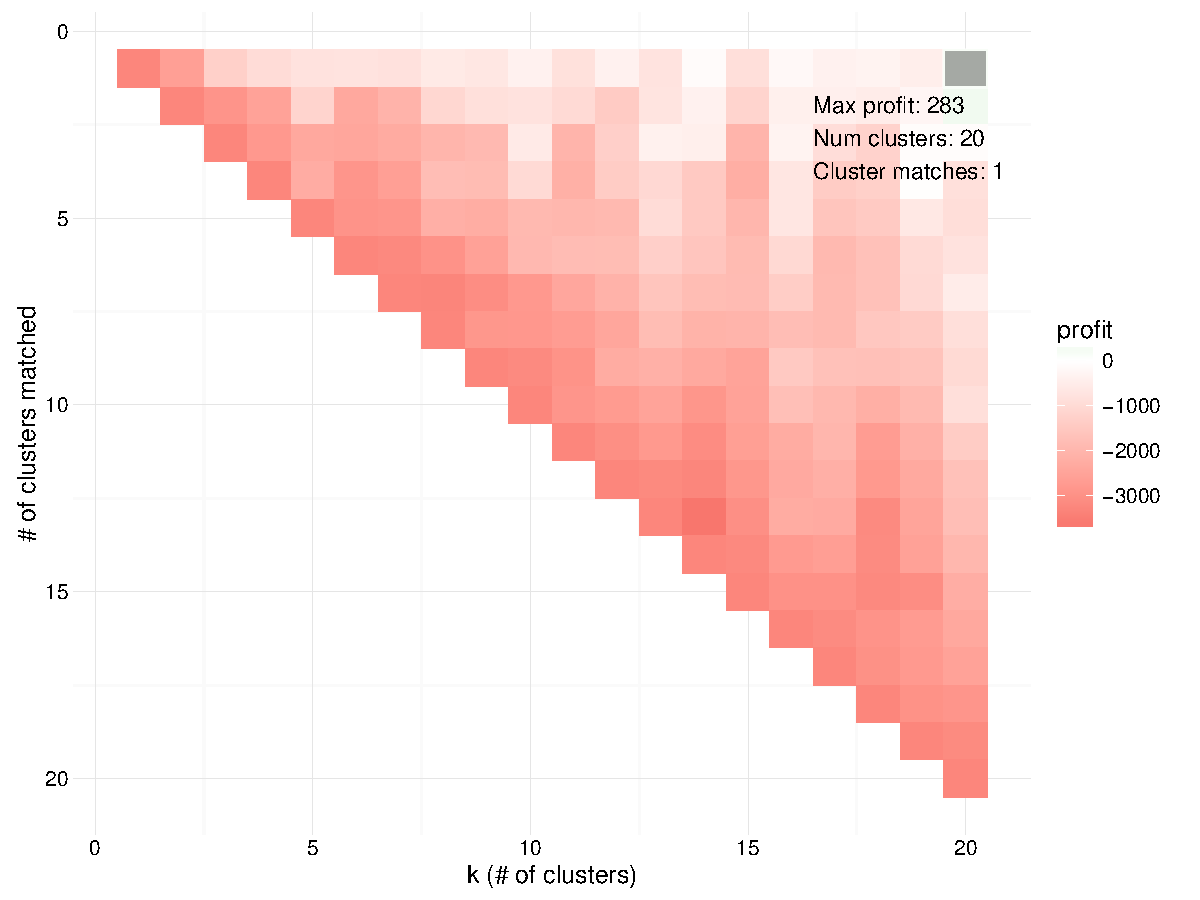
\includegraphics[scale=.5]{kmeans_profit1.pdf}
  \label{fig:kmeans_profit1}
\end{figure}

\begin{figure}[!htb]
  \centering
  \caption{Profitability of K-Means Matching, Data Set 2}
  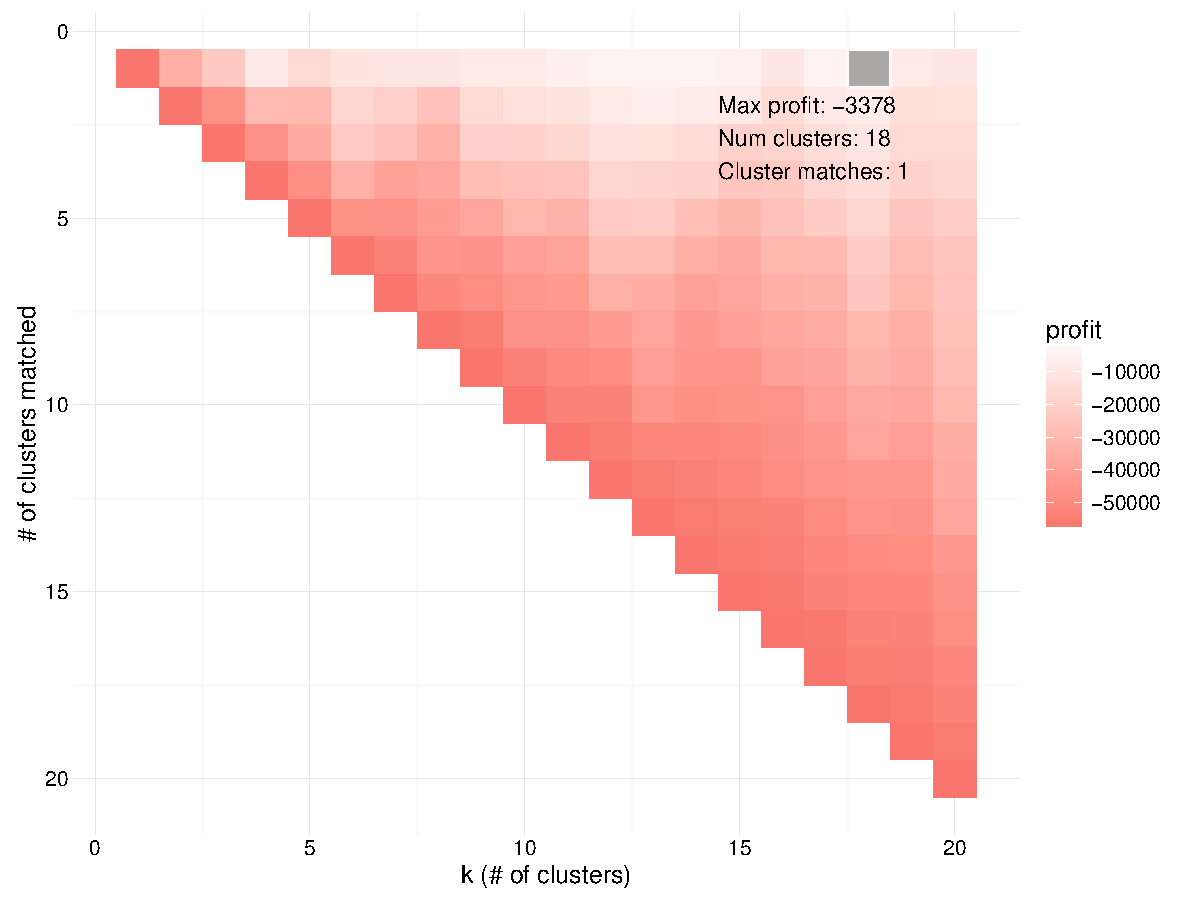
\includegraphics[scale=.5]{kmeans_profit2.pdf}
  \label{fig:kmeans_profit2}
\end{figure}


\section{K-Nearest-Neighbors Matching}

\subsection{Significant Variables}
To begin our exploration of the K-Nearest-Neighbors matching, we look to discover variables that significantly predict a customer's spend.  Our tool of choice here is the gamma lasso regression provided by the \textit{gamlr} package in R.  Using it, we regress \textit{spend} on all other variables (removing only \textit{machine\_id}) for both the original customer list (without \textit{ecom\_index}) and the new customer list containing \textit{ecom\_index}.  Then we look at the variables chosen by the using the AIC and BIC decision criteria (see \vref{tab:series_coefs}).  Note that the BIC substitutes \textit{retail\_index} with \textit{ecom\_index} when moving to the new data-set.  Moreover, the AIC chooses both variables when available.  We also curated our own covariates which we label as \textit{manual}.

% latex table generated in R 3.2.3 by xtable 1.8-2 package
% Tue Apr 12 04:02:36 2016
\begin{table}[ht]
\centering
\caption{Significant Coefficients by Series} 
\label{tab:series_coefs}
\begin{tabular}{rlll}
  \hline
 & No ecom\_index (BIC) & With ecom\_index (BIC) & With ecom\_index (AIC) \\ 
  \hline
1 & census\_region2 & census\_region2 & census\_region2 \\ 
  2 & household\_size6 & household\_size6 & household\_size6 \\ 
  3 & hoh\_oldest\_age2 & hoh\_oldest\_age2 & hoh\_oldest\_age2 \\ 
  4 & household\_income6 & household\_income6 & household\_income6 \\ 
  5 & retail\_index & ecom\_index & retail\_index \\ 
  6 &  &  & ecom\_index \\ 
   \hline
\end{tabular}
\end{table}


\subsection{Customer Spend Cutoff}
The next step in our K-Nearest-Neighbors algorithm is to select a spending cutoff that maximize profits.  The spending cutoff defines which of the existing customer profiles (from the \textit{cust2} data-set) will be used to match customers from the target data set.  As we saw from \vref{fig:cust_spend_cdf,fig:cust_spend_hist}, customer spending varies widely across the population.  Therefore, setting the threshold higher results in fewer existing customers to use for matching.  Intuitively speaking setting the cutoff high may be desirable if high-spend customers tend to cluster together.  However, if high-spend customers are hard to predict, then it may be more desirable to set the threshold lower hoping that lower-spend customers cluster together and, as a group, contribute greatly to profitability.

To perform this exercise, we use the kNN algorithm in the \textit{FNN} package to find target customers close to our existing customers (defined by the matching cutoff).  Using it, we vary both the number of nearest neighbors and the cutoff using the 2.5\% percentile steps in customer spend (see \vref{tab:cutoffs} for reference).  At each point in the search we calculate the profit, the fraction of all potential customers captured, the fraction of total possible revenue captured, and, finally, the fraction of the matched targets that are actually customers.  This sequence was performed for each of the following series':
\begin{itemize}
\item \textit{Orig. (AIC)} - is missing \textit{ecom\_index} and uses AIC to select covariates;
\item \textit{Manual} - has \textit{ecom\_index} and uses a manual covariate selection;
\item \textit{AIC} - has \textit{ecom\_index} and uses AIC to select covariates;
\item \textit{BIC} - has \textit{ecom\_index} and uses BIC to select covariates.
\end{itemize}

From \vref{fig:threshold_max_profit,tab:series_max} we see that most profitable strategy is to use the AIC selected covariates with the \textit{ecom\_index} setting both the threshold to a rather low value of \$8.72 and selecting the 3 closest neighbors to these values.  With this value we capture $\sim83\%$ of all customers and $\sim85\%$ of potential revenue with $\sim51\%$ of all targeted people spending money.  This strategy yields a healthy profit of \textbf{\$5,028.85}.  However it is very sensitive to the choice of \textit{k} being optimal.  Using the manually or BIC chosen coefficients yields a less sensitive approach that still yields a good fraction of customers and revenue along with a profit of \textbf{\$4,800.48} and \textbf{\$4,541.70} respectively.

\begin{figure}[!htb]
  \centering
  \caption{Max Profits vs. Threshold/K-Value by Series}
  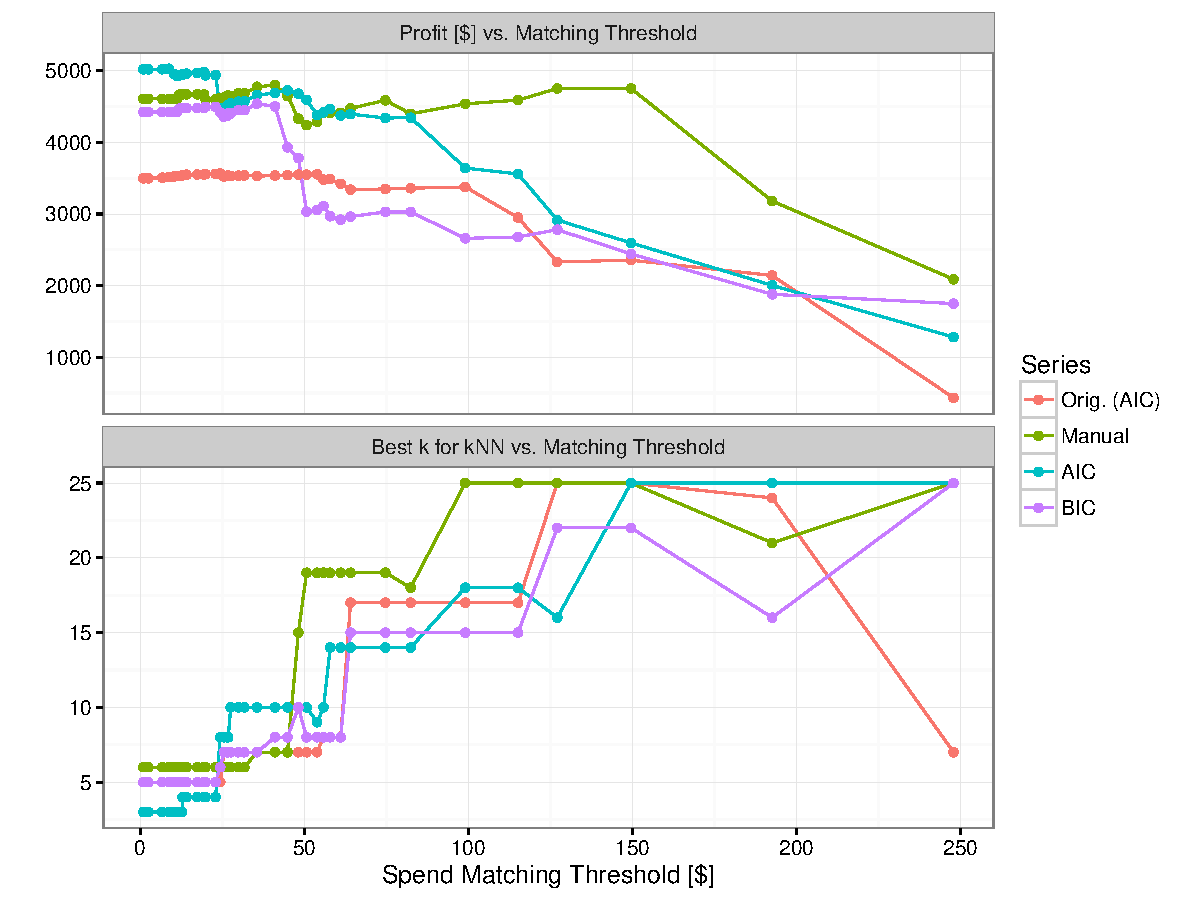
\includegraphics[scale=.75]{threshold_max_profit2.pdf}
  \label{fig:threshold_max_profit}
\end{figure}

% latex table generated in R 3.2.3 by xtable 1.8-2 package
% Tue Apr 12 03:01:59 2016
\begin{table}[ht]
\centering
\caption{Best matching threshold by explanatory variables} 
\label{tab:series_max}
\begin{tabular}{lrlrrrrr}
  \hline
Series & MatchingThreshold [\$] & Threshold \% & Best NN Choice & Profit [\$] & \% Cust Captured & \% Revenue Captured & \% Cust Matched \\ 
  \hline
Manual & 41.10 & 57.5\% &   7 & 4800.48 & 79.09 & 82.79 & 43.72 \\ 
  AIC & 8.72 & 10\% &   3 & 5028.85 & 82.73 & 85.17 & 51.41 \\ 
  BIC & 35.62 & 55\% &   7 & 4541.70 & 76.36 & 80.04 & 37.67 \\ 
   \hline
\end{tabular}
\end{table}



\subsection{Conclusions}
Ultimately, having the \textit{ecom\_index} covariate helps us quite a bit with our targeting.  Even with the 6.5x difference in the targeting price we are able to obtain higher profits -- up to \textbf{\$5,028.85} vs. \textbf{\$3,565.78}.  When we begin to look at the other measures like fraction of revenue and customers captured as well as the fraction of customers matched it's quite clear that the value of the \textit{ecom\_index} is quite striking (see \vref{fig:profits} for more measures by series in addition to profitability).  Therefore, in light of all of these benefits, \textbf{we would be willing to switch to the new DMP even at the higher cost.}

\begin{figure}[!htb]
  \centering
  \caption{Various Match Measures by Series}
  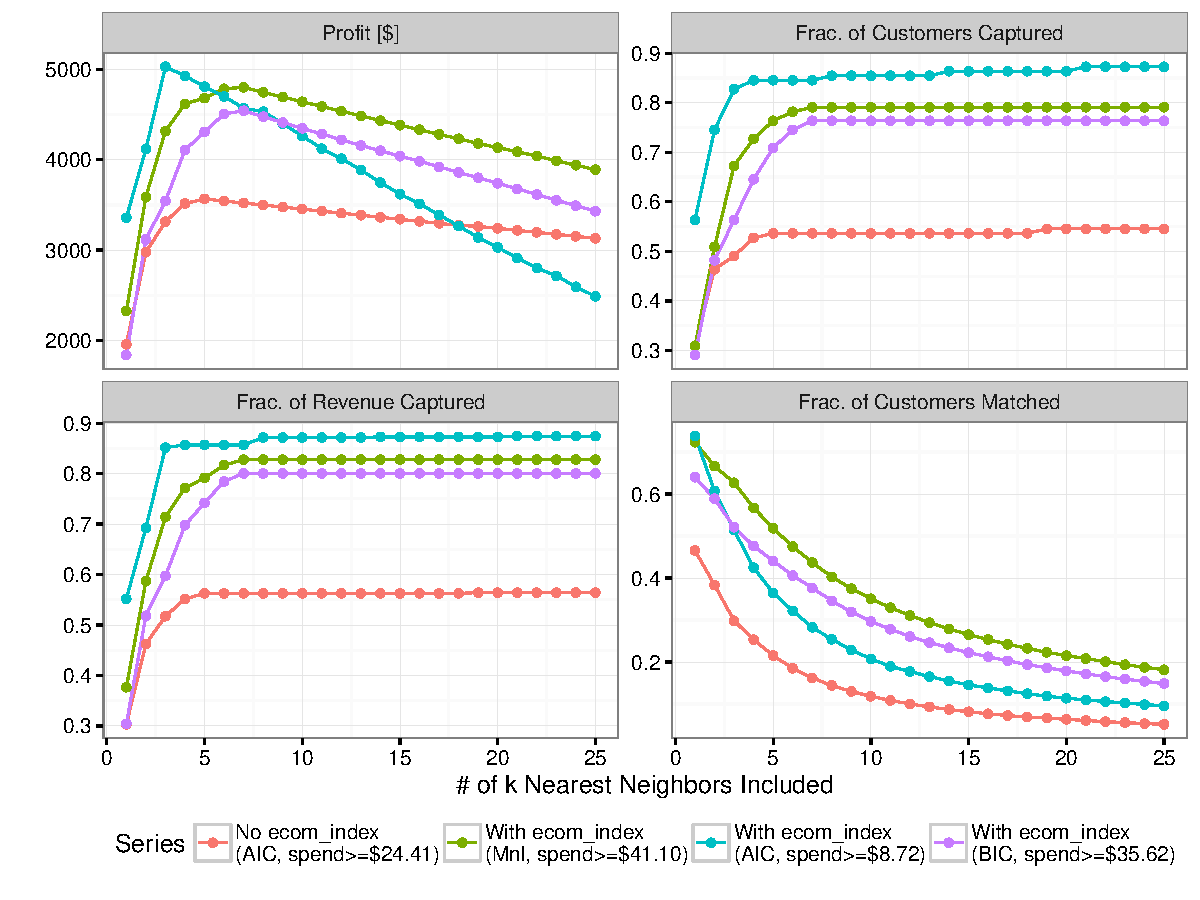
\includegraphics[scale=.75]{profits2.pdf}
  \label{fig:profits}
\end{figure}

\section{Targeting the Entire Data Set} % Question 2
We would pursue the entire target file under two conditions. First, the cost per person would need to be sufficiently low such that our status-quo profit from Part 1 would not suffer from targeting everyone. Second, there would need to be a “network” benefit to our business from having a larger user base on our platform. An example would be if were operating LinkedIn and we wanted to get more premium subscribers (i.e. people who spend money on our site) \textit{and} we also wanted to augment the general user base so that people on our site can develop a deeper professional network. Similarly, if we were operating an online dating service, we would not only be interested in getting the people who will buy a premium subscription. We would also want to augment the number of “regular” users so that our dating service has a deep pool of online connections between users.

With respect to the cost of targeting, we would pursue the entire target file audience if the cost were less than or equal to \textbf{\$0.10} per person.

In order to arrive at this solution, we created a vector of the cost per person with a range of \$0 to \$5 in increments of 10 cents. We then calculated the profit from pursuing everyone on the target list at each cost per person. At a cost of \$0.10 per person, our expected profit from targeting the whole file would be \$4,611.23. This is similar to the profit that we were able to achieve in Part 1 when we matched with the DMP that charges \$3.25 per person.

As shown in \cref{fig:Profit_Grid} below, the profit from pursuing everyone in the target file decreases with the cost per person. Therefore, the cost would need to be sufficiently low (less than \$0.10 per person in our case) for the 'blanket' approach of targeting everyone to be attractive. 

Of course, if targeted matching were available at \$0.10 or less per person, we could achieve even higher short-term profits through targeted marketing relative to a blanket approach. Therefore, the second condition for using a blanket approach is that we would need to have a network motivation (such as broadening the connections between users of our site) for this blanket approach to make sense from a business perspective. A broader network of users would be valuable in terms of long term profits because it could increase the advertising revenue on our site over the long run.

\begin{figure}[!htb]
  \centering
  \caption{Profits from Targeting Entire File by Cost}
  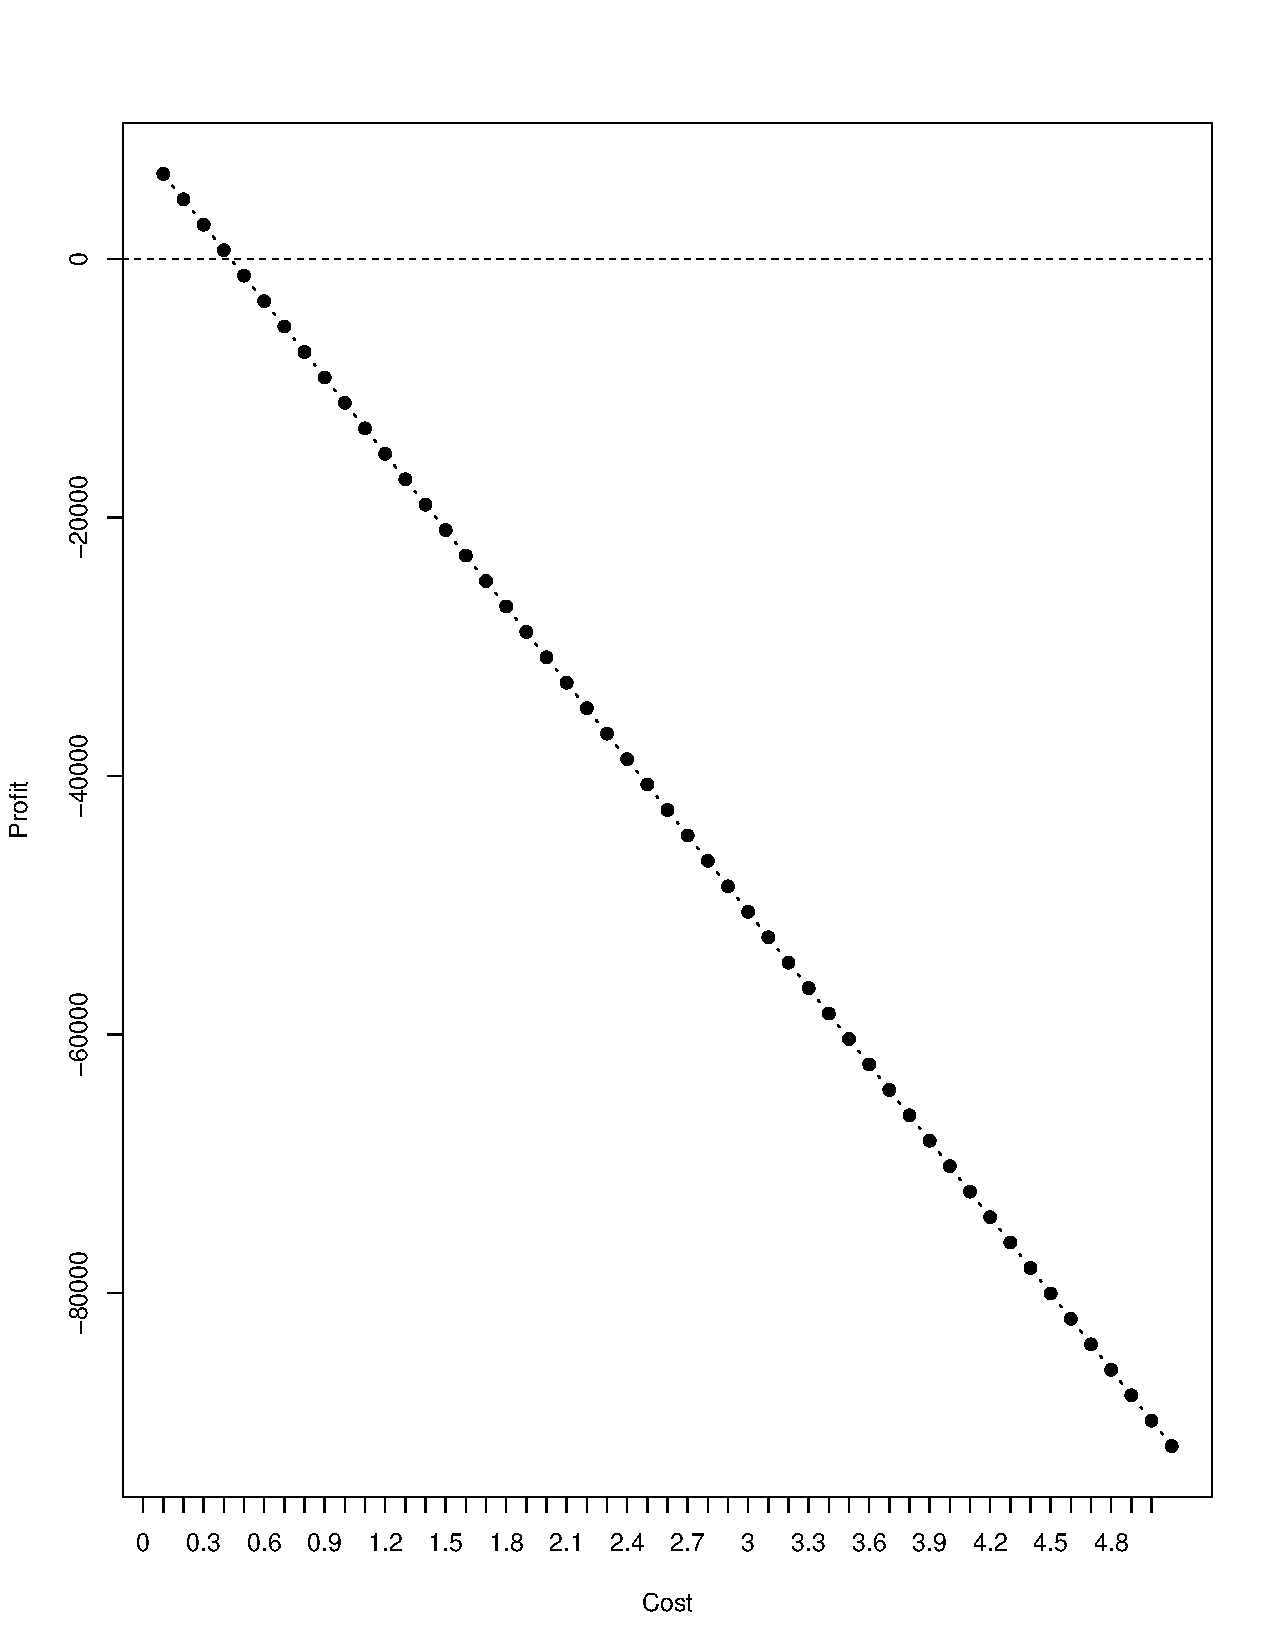
\includegraphics[scale=.5]{Profit_Grid.pdf}
  \label{fig:Profit_Grid}
\end{figure}

\clearpage
\section{Appendix}
% latex table generated in R 3.2.4 by xtable 1.8-0 package
% Tue Apr 12 09:38:48 2016
\begin{table}[ht]
\centering
\caption{Non-Zero Spend Quantiles} 
\label{tab:cutoffs}
\begin{tabular}{rrrr}
  \hline
Percentile & Spend & Percentile & Spend \\ 
  \hline
5 & 2.52 & 55 & 35.62 \\ 
  10 & 8.72 & 60 & 44.92 \\ 
  15 & 11.17 & 65 & 50.72 \\ 
  20 & 12.72 & 70 & 55.89 \\ 
  25 & 14.14 & 75 & 61.12 \\ 
  30 & 19.46 & 80 & 74.75 \\ 
  35 & 22.98 & 85 & 99.11 \\ 
  40 & 25.54 & 90 & 127.15 \\ 
  45 & 26.84 & 95 & 192.64 \\ 
  50 & 29.94 &  &  \\ 
   \hline
\end{tabular}
\end{table}


\end{document}

% \input{.tex}

% \begin{figure}[!htb]
%   \centering
%   \caption{}
%   \begin{subfigure}[b]{0.49\textwidth}
%     \caption{}
%     \includegraphics[width=\textwidth]{.pdf}
%     \label{fig:}
%   \end{subfigure}
%   \hfill
%   \begin{subfigure}[b]{0.49\textwidth}
%     \caption{}
%     \includegraphics[width=\textwidth]{.pdf}
%     \label{fig:}
%   \end{subfigure}
% \end{figure}

% \begin{figure}[!htb]
%   \centering
%   \caption{}
%   \includegraphics[scale=.5]{.pdf}
%   \label{fig:}
% \end{figure}